The measurement at the heart of this thesis can only be understood within the context of a vast amount of preceeding theoretical and experimental work. I have tried to condense and summarize key concepts that will motivate the central measurement's strategy and results. This chapter begins with a brief summary of the Standard Model itself, first describing fundamental particles and their forces before delving into a succinct mathematical formulation. Next, the chapter discusses the history of the Standard Model and crucial tests of the theory up until current work at the Large Hadron Collider (LHC). The next section outlines some of the recent physics analyses at the LHC with a focus on Higgs boson measurements. Finally, I introduce my thesis' main focus, fiducial cross-section measurements of VBF Higgs bosons decaying into two $W$-bosons.

\section{Standard Model}

The Standard Model (SM) is one of the most successful scientific theories to date. Its predictions encompass all of the visible universe and continue to undergo careful testing. The SM combines three forces---electromagnetic, weak, and strong---but it is not complete. One known force, gravity, is not included in the Standard Model and further questions, like dark matter and dark energy, remain. 

\subsection{Particles and forces}
The particles we define in high energy physics are the most minute portions of observable matter. They are generally considered point-like, have no internal structure, and cannot be further split. Each particle we can define has a unique set of quantum numbers and its own anti-particle (with the same mass and spin, but opposite electrical charge and quantum numbers).

Particles can be sorted into two distinct groups: bosons, with integer spin, and fermions, with half-integer spin. Bosons are `force carriers' meaning they are exchanged any time particles interact. Fermions are at the heart of all conventional matter and can be split further into two categories, leptons and quarks. Quarks have fractional charge (in units of the proton's charge) and interact strongly, while leptons have integer charge and interact solely through the weak or electromagnetic forces. Both quarks and leptons are made of three generations of particles, each heavier than the previous. Charts showing quark/lepton families and their key quantum numbers are shown below in Figure \ref{fig:SMparticles}. Each generation of quarks and leptons contains a particle doublet. Each lepton doublet contains a charged lepton and a neutrino while each quark doublet contains one $+2/3$ charged particle and one with a $-1/3$ charge. Each lepton and quark also has an anti-particle. All conventional, stable matter is made from the first generation of quarks and leptons.

There are four gauge bosons and one scalar boson predicted through the Standard Model. These correspond to three fundamental forces in nature (the fourth, gravity, is so small on the scale of particle interactions as to not be considered). The strongest force on the subatomic scale works primarly to bind quarks together to form composite particles like protons or neutrons. The electromagnetic force is mediated by the photon. This force accounts for all electric interactions like that between an electron an an atomic nucleus. Finally, the weak force is mediated by exchange of massive $W$ and $Z$ bosons. The $\beta$-decay of nuclei (mediated by $W$ bosons) is a weak interaction process. The final boson predicted by the Standard Model is the Higgs boson. The only scalar boson, it has no charge or intrinsic spin. The Higgs gives mass to all other particles through Spontaneous Symmetry Breaking, which will be described in later sections.
\begin{figure}[H]
	\centering
    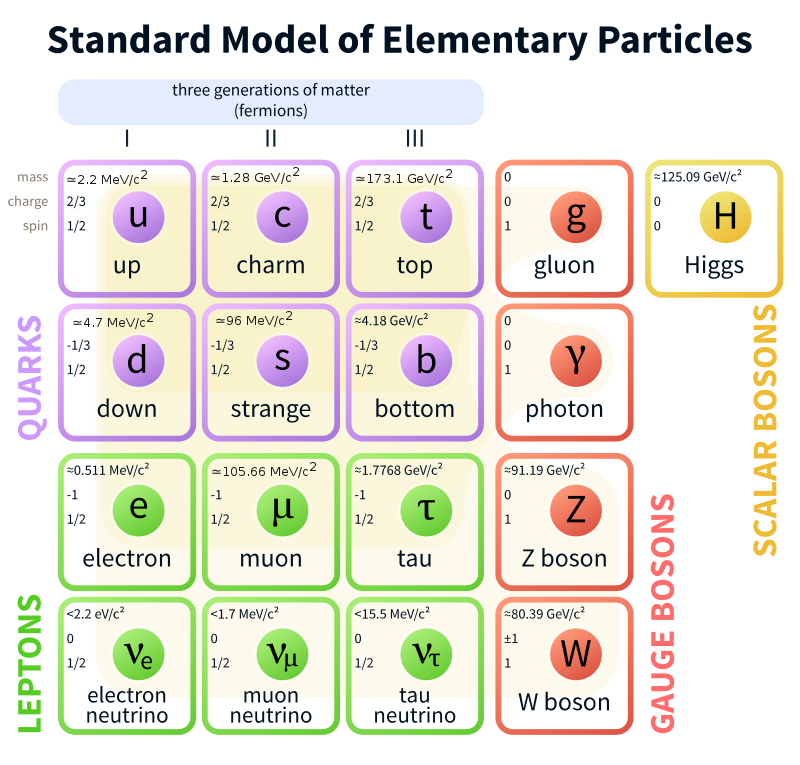
\includegraphics[width=0.7\textwidth] {Pictures/SMparticles.png}\hspace{1cm}
    \caption{Three generations of quarks and leptons are shown along with all SM bosons \cite{PDG}}
    \label{fig:SMparticles}
\end{figure}
Photons are massless, spin-1 particles and mediate all electromagnetic interactions. They couple directly to any particle with electric charge, leptons and $W$ bosons but not neutrinos. Since the photon is massless, the electromagnetic force can operate on infinitely long scales but its force decreases with $1/r^2$.
 
Gluons are massless particles with no electric charge and spin-1. They couple to color charges, which are a property only of quarks and gluons. Each quark has one of three colors (RGB). Colors ore conserved `charges' similar to electric charge. Quarks are never found alone as they couple so strongly to one another as to be confined in groups. These groups are ``color-confined" meaning the quarks contain colors which add up to a color neutral sum.  Gluons also have color charge and can thus couple to each other. This makes the strong force distinct from the electromagnetic and has implications for long-distance interactions.
 
The $W$ and $Z$ bosons, unlike gluons and photons, are massive. However, like their other gauge boson counterparts, they have spin-1 and mediate interactions. The $W^{\pm}$ mediates charged-current interactions which can violate flavor conservation between quarks and/or leptons and their neutrinos. The $Z$ mediates neutral-current interactions which conserve flavor. The $W^{\pm}$ bosons contain electric charge so can interact through EM interactions, as well. In addition, $W$ and $Z$ bosons contain weak charge (as do all fermions) so can self-couple as well as couple with all fermions. 
 
The Higgs boson will be further motivated and described in later sections but suffice to say it is a massive, spin-0 particle which couples to all particles with mass (including itself). It does not mediate any force but it is still an integral part of the Standard Model.  

\subsection{Gauge Invariance}
According to Noether's theorem, for every continuous transformation of a field that leaves the Lagrangian invariant, there is a conserved current. In other words, symmetries found in physical theories lead to conservation laws (and vice-versa). The Standard Model is a gauge theory built on symmetries; all interactions between particles result from requiring the theory to be invariant under local gauge transformations. Each part of the Standard Model, from quantum electrodynamics (QED) to quantum chromodynamics (QCD), is a gauge theory on its own. Each part has gauge invariance symmetries. In this section I step through the basic mathematic formalism for QED, QCD, and the combined electro-weak theory to illustrate the physical ramifications of gauge invariance and set the stage for the Higgs mechanism. The following sections are written with guidance from \cite{HalzenMartin}. 

\subsubsection{Quantum Electrodynamics}
Quantum electrodynamics (QED) is the first, and simplest, physical gauge theory, describing how light and matter interact even under relativistic conditions. The theory produces extremely good agreement with experiment due to the success of perturbative QED calculations. Entire textbooks are dedicated to QED formalism and predictions. Here I will highlight only the effects of its local gauge invariance symmetry and generating the full QED Lagrangian beginning with the Dirac Lagrangian of a free fermion. 

The Dirac Lagrangian describes a free fermion of mass \textit{m}
\begin{equation}
\mathcal{L} = i \psi \gamma^\mu \partial_ \mu \psi - m\bar{\psi}\psi,
\end{equation}
where $\psi$ is a Dirac spinor and $\gamma^\mu$ represent the Dirac matrices. To demonstrate local gauge invariance we need to transform
\begin{equation}
\psi(x) \rightarrow e^{i\alpha(x)}\psi(x), 
\end{equation}
where $\alpha(x)$ depends on space and time arbitrarily. Directly substituting this into our Lagrangian shows that $\mathcal{L}$ is not invariant, due to the $\partial_\mu$ term 
\begin{equation}
\partial_\mu \psi \rightarrow e^{i\alpha(x)}\partial_\mu\psi + ie^{i\alpha(x)}\partial_\mu \alpha.
\end{equation}
In order to mandate the theory is invariant we need to change this term to the ``covariant derivative" $D_\mu$ which transforms 
\begin{equation}
D_\mu\psi \rightarrow e^{i\alpha(x)}D_\mu\psi. 
\end{equation}	 
The ``covariant derviative" must contain a vector field $A_\mu$ and this field must transform so as to cancel with the unwanted part of the transformed $D_\mu$ in order to transform as required by gauge invariance. 
\begin{equation}
D_\mu \equiv \partial_\mu - ieA_\mu
\end{equation}
where 
\begin{equation}
A_\mu \rightarrow A_\mu + \frac{1}{e}\partial_\mu \alpha.
\end{equation}
Now the original Dirac equation is replaced with the following:
\begin{equation}
\mathcal{L} = \bar{\psi}(i\gamma^\mu\partial_\mu-m)\psi + e\bar{\psi}\gamma^\mu\psi A_\mu.
\end{equation}
By requiring local gauge invariance we have introduced a gauge field $A_\mu$ which couples to the Dirac particle just as the photon. In fact, if we take this as the photon gauge field and so add a kinetic energy term (which is also local gauge invariant!) we find the Lagrangian of QED: 
\begin{equation}
\mathcal{L} = \bar{\psi}(i\gamma^\mu\partial_\mu-m)\psi + e\bar{\psi}\gamma^\mu\psi A_\mu -\frac{1}{4} F_{\mu\nu}F^{\mu\nu}.
\end{equation}
One can also see that adding a mass term to the Lagrangian for the new field ($\frac{1}{2}m^2A_\mu A^\mu$) would break gauge invariance, indicating the photon must be massless. From the free fermion Lagrangian, imposing local gauge invariance leads to the full interacting field theory of QED. This is not a curiosity but an essential component of the theory, and the use of local gauge symmetry in deriving particle interactions does not end here.

\subsubsection{Quantum chromodynamics}
Quantum chromodynamics differs from QED in a few crucial ways. Since quark color fields exist, the QED $U$(1) gauge group is replaced with $SU$(3) and the free Lagrangian contains indices $j$ to denote the three color fields: 
\begin{equation}
\mathcal{L} = \bar{q}_j(i\gamma^\mu\partial_\mu - m)q_j.
\end{equation}
QCD also carries three quark flavors, which will be ignored here for simplicity. The QCD group is non-Abelian since not all generators of the group commute with each other. These generators will be defined as $T_a$ where $a=1,...,8$ and are linearly independent traceless $3\times3$ matrices (the Gell-Mann matrices $\lambda_a$ are conventional). The local color phase transformation required is thus 
\begin{equation}
q(x) \rightarrow e^{i\alpha_a(x)T_a}q(x).
\end{equation}
We can consider an infinitesimal phase transformation as 
\begin{equation}
\begin{split}
q(x) \rightarrow [1+i\alpha_a(x)T_a]q(x), \\ 
\partial_uq \rightarrow (1+i\alpha_aT_a)\partial_\mu q + i T_a q \partial_\mu \alpha_a.
\end{split}
\end{equation}
Just as in the QED example, the last line breaks the invariance of $\mathcal{L}$, and we can proceed similarly by introducing a new gauge field (or in this case eight) called $G_\mu^a$ which transform as
\begin{equation}
G_\mu^a \rightarrow G_\mu^a - \frac{1}{g}\partial_\mu\alpha_a - f_{abc}\alpha_b G_\mu^c.
\end{equation}
The last term added here is to cope with the non-Abelian nature of QCD.\footnote{Non-Abelian here means the generators $T_a$ commute with each other.} Just as in QED this invariance forms a covariant derviative:
\begin{equation}
D_\mu = \partial_\mu + i g T_aG_\mu^a.
\end{equation}
Replacing the derivative in our Lagrangian and adding a gauge invariant energy term for each of the $G_\mu^a$ fields ($\frac{1}{4}G_{\mu\nu}^a G^{a \, \mu\nu}$) yields the final gauge invariant QCD Lagrangian:
\begin{equation}
\mathcal{L} = \bar{q}(i\gamma^\mu\partial_\mu - m)q - g(\bar{q}\gamma^\mu T_aq)G_\mu^a-\frac{1}{4}G_{\mu\nu}^aG^{a \, \mu\nu}.
\end{equation}
Just as in the QED case, imposing local color phase invariance produced 8 new interacting fields with coupling $g$. These are the gluon fields and just like photons, local gauge invariance requires them to be massless. Unlike the QED case, this Lagrangian's new kinetic term includes self-interaction between the gauge bosons - another key feature of QCD that is mandated by local color phase invariance. Gluons themselves must carry color charge and therefore they self-couple. The structure of these self coupling terms and their single coupling strength $g$ are uniqely determined by gauge invariance. 

\subsubsection{Electroweak unification}
Thus far, I have summarized the theoretical backgrounds for symmetries (and so conserved quantities) in both quantum electrodynamics and chromodynamics. The weak force is the final Standard Model force and weak interactions are mediated by $Z$ and $W$ bosons. Unlike the gluons and photons of QCD and QED, these gauge bosons are massive. This is explained through spontaneous symmetry breaking of the electroweak force, which is outlined in the following section. Assuming that $W$/$Z$ bosons are massive, the weak force can be combined with QED and a central electroweak force (with its associated symmetries) can be described. 

The weak neutral current $J_\mu^{NC}$ and weak charged currents ($J_\mu$, $J_\mu^\dagger$) can form a symmetry group for weak interactions. The charged currents correspond to the charged weak interaction through $W^\pm$ bosons while the neutral current is associated with the $Z$ boson:
\begin{equation}
\begin{split}
J_\mu=\bar{\nu_L}\gamma_\mu\nu_L, \\
J_\mu^\dagger =\bar{e_L}\gamma_\mu\nu_L
J_\mu^3=\frac{1}{2}\bar{\nu_L}\gamma_\mu\nu_L-\frac{1}{2}\bar{e_L}\gamma_\mu e_L,
\end{split}
\end{equation}
where $L$ denotes that these are left-handed spinors. The charged currents can be written as a doublet using the Pauli spin matrices $\tau_i$ where $\tau_\pm=\frac{1}{2}(\tau_1\pm i\tau_2)$ and
\begin{equation}
\chi_L=\begin{bmatrix}
        \nu  \\
        e^-
        \end{bmatrix}
\end{equation}
as 
\begin{equation}
\begin{split}
J_\mu^+(x)=\bar{\chi_L}\gamma_\mu\tau_+\chi_L, \\
J_\mu^+(x)=\bar{\chi_L}\gamma_\mu\tau_-\chi_L, \\
J_\mu^3(x)=\bar{\chi_L}\gamma_\mu\frac{1}{2}\tau_i\chi_L \textnormal{ with } i=1,2,3
\end{split}
\end{equation}
The corresponding charge $T^i=\int J_0^i(x)d^3x$ can be introduced so we have an $SU$(2)$_L$ algebra
\begin{equation}
[T^i,T^j]=i\epsilon_{ijk}T^k.
\end{equation}
Unfortunately while these currents create an $SU$(2) group, they do not correspond with the weak neutral current symmetry in an obvious way. Unlike the charged currents, the neutral current has a right-handed component. One way to attain the expected symmetry is to add in the electromagnetic current, as it is a neutral current with components
\begin{equation} 
j_\mu^{em}(x)=-\bar{e_R}\gamma_\mu e_R-\bar{e_L}\gamma_\mu e_L
\end{equation}
so the the electromagnetic current $j_\mu$ can be written using the coupling $e$
\begin{equation}
j_\mu=e j_\mu^{em} = e\bar{\psi}\gamma_\mu Q\psi
\end{equation}
with $Q$ the charge operator and generator of the $U$(1) symmetry group of EM. In order to ``save" the symmetry of the weak neutral current, we can define an electromagnetic current $j_\mu^Y$, or the weak hypercharge current, that is unchanged by $SU$(2)$_L$ transformations. We define a weak hypercharge $Y$ and its current $j_\mu^Y$
\begin{equation}
\begin{split}
Q=T^3+\frac{Y}{2}, \\
j_\mu^Y =\bar{\psi}\gamma_\mu Y \psi.
\end{split}
\end{equation}
The combined current 
\begin{equation}
j_\mu^{em} = J_\mu^3+\frac{1}{2}j_\mu^Y
\end{equation}
now generates the symmetry group $U$(1)$_\gamma$ and so the electromagnetic interaction and weak interaction are combined into one $SU$(2)$_L$ $\times$ $U$(1)$_\gamma$ group. While unified in this way, the two forces still have independent coupling strengths. This brief introduction into electroweak unification is not the complete picture---EM and weak \textit{interactions} still have to be unified. In the Standard Model framework, electroweak currents just have to be coupled to vector bosons to complete unification. In the electroweak $SU$(2)$_L$ $\times$ $U$(1)$_\gamma$ group, there is an isotriplet of vector fields $W_\mu^i$ coupled with strength $g$ to the weak isospin current $J_\mu^i$, while a single vector field $B_\mu$ is coupled to the weak hypercharge current $j_\mu^Y$ with strength $g'/2$. The electroweak Lagrangian interaction term can thus be defined:
\begin{equation}
-i g (J^i)^\mu W_\mu^i-i\frac{g'}{2}(j^Y)^\mu B_\mu .
\end{equation}
This summary of the unified electroweak force will be the starting point for a derivation of the Higgs boson and an explanation for mass of the weak force's vector bosons (and all the fermions). The electroweak theory is unique in its calculability even at higher order scales. Consequently, theoretical uncertainties are relatively low and many deviations from theory could potentially be observed at current energy scales. The measurement central to my thesis probes for such discrepancies in electroweak theory. The mechanisms for this will be explained in the last section in this chapter. 

\subsubsection{Spontaneous Symmetry Breaking}
Unlike QED and QCD, the weak force is mediated by massive gauge bosons. We therefore can not apply the same gauge invariance prescription that we did in the last sections. If a mass term is added to the Lagrangian, we break the gauge invariance we aimed to find. If we instead ignore the gauge invariance and add a mass term to the Lagrangian, all predictive power of the theory is lost due to unrenormalizable divergences. With ``spontaneous symmetry breaking" we can gain massive gauge bosons while maintaining the integrity of the theory. In this section, I first describe the "spontaneous symmetry breaking" mechanism is terms of an Abelian theory composed of complex scalar fields to illustrate the overall strategy. This mechanism is then applied to the non-Abelian electroweak theory to gain massive weak gauge bosons, $W^{\pm}$ and $Z$, with the Higgs field appearing as a `spontaneous' result.

The Lagrangian for a $U$(1) gauge symmetry can be given as 
\begin{equation}
\phi \rightarrow e^{i\alpha(x)}\phi.
\end{equation}
As in the QED case, we introduce a gauge field $A_\mu$ and covariant derivative $D_\mu = \partial_\mu - ieA_\mu$ to obtain the gauge invariant Lagrangian,
\begin{equation}
\mathcal{L} = (\partial^\mu+ieA^\mu)\phi^*(\partial_\mu-ieA_\mu)\phi-\mu^2\phi^*\phi-\lambda(\phi^*\phi)^2-\frac{1}{4}F_{\mu\nu}F^{\mu\nu}.
\end{equation}
In this example if $\mu^2>0$ we gain back the QED Lagrangian for a charged scalar particle of mass $\mu$ with an additional self-interaction term. However, if we take $\mu^2<0$ the potential $V(\phi^*\phi)=\mu^2\phi^*\phi-\lambda(\phi^*\phi)^2$ acquires a non-zero vacuum expectation value (v.e.v.) and there is a set of equivalent minima shown in Figure \ref{fig:HiggsPotential}. Choosing one of these minima spontaneously breaks the potential's rotational symmetry. We can perturbatively expand the field about a minimum through
\begin{figure}[H]
    \centering
    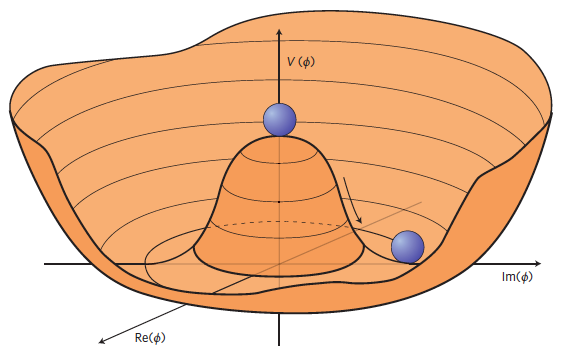
\includegraphics[width=0.5\textwidth] {Pictures/HiggsPotential.png}\hspace{1cm}
    \caption{Higgs potential when $\mu^2<0$, choosing a minima spontaneously breaks the $U$(1) rotational symmetry \cite{HiggsPotential}}.
    \label{fig:HiggsPotential}
\end{figure}

\begin{equation}
\phi(x) =\sqrt{\frac{1}{2}[\nu+\eta(x)+i\xi(x)]}.
\end{equation}
We substitute this perturbation into the Lagrangian and gain
\begin{equation}
\mathcal{L}'=\frac{1}{2}(\partial_\mu\xi)^2+\frac{1}{2}(\partial_\mu\eta)^2-\nu^2\lambda\eta^2+\frac{1}{2}e^2\nu^A_\mu A^\mu-e\nu A_\mu \partial^\mu\xi-\frac{1}{4}F_{mu\nu}F^{\mu\nu} + \textnormal{interaction terms}.
\end{equation}
Three particles emerge here: a massless Goldstone boson $\xi$, a massive vector $A_\mu$ with $m_A=e\nu$, and a massive scalar $\eta$ with $m_\eta=\sqrt{2\lambda\nu^2}$. However, the number of particles does not correspond to the expected polarization degrees of freedom expected. A longitudonal polarization was added, creating an unphysical field, and injecting extra degrees of freedom. To eliminate the unphysical field we can substitute a new set of fields:
\begin{equation}
\phi \rightarrow \sqrt{\frac{1}{2}(\nu+h(x))e^{i\theta(x)/\nu}}
\end{equation}
and 
\begin{equation}
A_\mu \rightarrow A_\mu + \frac{1}{e\nu} \partial_\mu\theta.
\end{equation}
Introducing these substitutions, the Goldstone boson field disappears and the new Lagrangian becomes 
\begin{equation}
\mathcal{L} = \frac{1}{2}(\partial_\mu h)^2 -\lambda\nu^2h^2+\frac{1}{2}e^2\nu^2A_\mu^2-\lambda\nu h^3-\frac{1}{4}\lambda h^4+\frac{1}{2}e^2A_\mu^2h^2+\nu e^2A_\mu^2h-\frac{1}{4}F_{\mu\nu}F^{\mu\nu}.
\end{equation}
Here the degrees of freedom before our substitutions remains the same and a massive boson $A_\mu$ is preserved along with a massive scalar $h$. The ``Higgs mechanism'' applied to a scalar field succeeded in creating a massive boson and determined the existence of a massive scalar boson. 

This same mechanism can be applied in the more complicated Standard Model electroweak field. Through electroweak symmetry breaking, we not only gain massive gauge bosons and a massive scalar boson (the Higgs) but we also gain a way to calculate testable Standard Model predictions for many other quantities. We start with the $SU$(2)$\times$$U$(1) gauge symmetry of electroweak interactions derived in the previous section. In order to gain masses for three gauge bosons and keep the photon massless, we need at least 3 degrees of freedom added, and a simple choice is to use the $SU$(2) doublet of scalar fields $\phi$, with four fields in an isospin doublet of weak hypercharge $Y=1$: 
\begin{equation}
\mathcal{L} =(D^\mu \phi)^\dagger(D_\mu\phi)-\mu^2\phi^\dagger\phi-\lambda(\phi^\dagger\phi)^2,
\end{equation}
where $\phi$ is a $SU$(2) doublet of complex scalar fields
\begin{equation}
\phi = \sqrt{\frac{1}{2}}\begin{bmatrix}
	\phi_1+i\phi_2  \\
	\phi_3+i\phi_4
	\end{bmatrix} .
\end{equation}
Local gauge invariance can be achieved just as in the $U$(1) case with the covariant derivative, though now a bit more complex:
\begin{equation}
D_\mu = \partial_\mu + ig \frac{\tau_a}{2}W_\mu^a
\end{equation}
with three gauge fields $W_\mu^a(x)$ and $a=1,2,3$. An infinitesimal transformation is defined as 
\begin{equation}
\phi(x)\rightarrow \phi'(x) = (1+i\alpha(x)\cdot\tau/2)\phi(x)
\end{equation}
and so the Lagrangian potential becomes
\begin{equation}
V(\phi) = \mu^2\phi^\dagger\phi+\lambda(\phi^\dagger\phi)^2.
\end{equation}
Once again if we choose the conditions $\mu^2<0$ and $\lambda>0$ there is rotational symmetry in our choice of vacuum expectation value. In this case, the choice of v.e.v. is limited. For the photon to remain massless, the vacuum must be invariant under $U$(1) (or electromagnetic) transformations, and not be charged in either direction (charge conservation). Thus the chosen minima to spontaneous break electroweak symmetry is
\begin{equation}
\phi_0  = \sqrt{\frac{1}{2}}\begin{bmatrix}
        0  \\
        \nu
        \end{bmatrix}.
\end{equation}
Next, substituting the vacuum expectation value $\phi_0$ for $\phi(x)$ and expanding perturbatively yields 
\begin{equation}
\phi(x) \rightarrow \begin{bmatrix}
        0  \\
        \sqrt{\frac{1}{2}(\nu+H(x))}
        \end{bmatrix}.
\end{equation}
Fully expanding this term in the Lagrangian gives a complex and illuminating result, the Goldstone bosons have been consumed and there is only a Higgs field ($H(x)$) remaining. Next, masses for the vector bosons are found from expanding one key parameter in the Lagrangian
\begin{equation}
|(-ig\frac{\tau}{2}\cdot W_\mu-i\frac{g'}{2}B_\mu)\phi|^2=\frac{1}{8}|\begin{bmatrix}
        gW_\mu^3+g'B_\mu && g(W_\mu^1-iW_\mu^2)  \\
        g(W_\mu^1+iW_\mu^2) && igW_\mu^3+g'B_\mu
        \end{bmatrix} \begin{bmatrix}
        0 \\
        \nu
        \end{bmatrix}|^2 .
\end{equation}
Expanding further and substituting $W^\pm =(W^1\pm iW^2)/\sqrt{2}$ gives the result
\begin{equation}
|(-ig\frac{\tau}{2}\cdot W_\mu-i\frac{g'}{2}B_\mu)\phi|^2= (\frac{1}{2}\nu g)^2W_\mu^+W^{-\mu}+\frac{1}{8}(W_\mu^3,B_\mu) \begin{bmatrix}
        g^2 && -gg' \\
        -gg' && g'^2
        \end{bmatrix} \begin{bmatrix}
        W^{\mu 3} \\
        B^\mu
        \end{bmatrix}.
\end{equation}
It is immediately clear that there is a mass term for the $W^\pm$, $M_W=\frac{1}{2}\nu g$. Masses for the photon and $Z$-boson are also apparent after expanding the last final term
\begin{equation}
\frac{1}{8}\nu^2(g^2(W^\mu_3)^2-2gg'W_\mu^3 B^\mu+g'^2B_\mu^2)=\frac{1}{8}\nu^2(gW_\mu^3-g'B_\mu)^2,
\end{equation}
and using the substitutions 
\begin{equation}
\begin{split}
A_\mu=\frac{g'W_\mu^3+gB_\mu}{\sqrt(g^2+g'^2)} \textnormal{ with  } M_A=0, \text{ and }\\
Z_\mu =\frac{gW_\mu^3-g'B_\mu}{\sqrt(g^2+g'^2)} \textnormal{ with  } M_Z=\frac{1}{2}\nu\sqrt(g^2+g'^2) .
\end{split}
\end{equation}

Now the Higgs field exists just as in the previous example and the theory contains a massive scalar boson and three massive vector gauge fields---one for each of the $W^\pm$ and $Z$ bosons. The Goldstone bosons degrees of freedom were used to give mass to the vector bosons. Choosing a ground state and so breaking the gauge symmetry does not eliminate this symmetry altogether, since the theory is still renormalizable. Fermion masses can also be derived from their interactions with the Higgs boson using this Lagrangian. These derivations can be used to predict masses of bosons and fermions and couplings to the Higgs boson. It is important to note that the Higgs mechanism gives mass to all fermions and massive gauge bosons, but it does not determine what the Higgs mass ought to be. This is left as an empirical input to the theory that can then be used to calculate other observables. 

The Standard Model has been proven over decades to be an incredibly robust theory. Since 2010, the Large Hadron Collider has become its key testing ground. 

\section{LHC Physics/Phenomenology}
The Large Hadron Collider (LHC) is the foremost Standard Model testing ground, and the proton-proton collisions recorded with the ATLAS, CMS, ALICE, and LHCb detectors have demonstrated the breadth and accuracy of the theory. Fermion and gauge boson masses and couplings, including the mass of the Higgs boson, have been measured with high precision. In the next chapter, the mechanics of the LHC and ATLAS detector will be discussed. Here I will introduce the motivations and observations of LHC physics. This section will begin with the mechanics of proton-proton collisions and their decay products, then discuss the concept of decay cross-sections, and finally focus more closely on the Higgs boson and its properties.

One of the LHC's central goal was to discover the missing Standard Model Higgs boson. The protons in the LHC collide at a center-of-mass energy of 13 TeV, but began at half that in 2010. The electroweak symmetry breaking scale was theoretically known to be between 100--1000 GeV, and so probing at 7 TeV provided near certainty of finding either the Higgs or an inconsistency in the Standard Model. The motivation for a proton collider was multifaceted. Foremost, using the tunnels built for the electron-positron detector LEP with protons allows the collider to reach higher energies, as protons do not lose as much energy to synchroton radiation as electrons. However, proton collisions have added complexity from their component quarks. Each parton (quark or gluon in the proton) carries some fraction of the momentum of the proton described by parton distribution functions. 

Figure \ref{fig:protonproton} shows a proton-proton collision schematic. In this example the hard process comes from the up quark in each proton \cite{Butterworth}. ``Hardness" refers to the fraction of proton momentum involved in the collision. In contrast, ``soft" collisions are those from remaining partons in each proton and usually involve low momentum transfer. These soft collisions are considered the underlying event shown in the Figure \ref{fig:protonproton}. Parton scattering is the most common hard process at the LHC by far due to the high density of gluons in the proton and the scale of QCD couplings above electroweak coupling strength. 
\begin{figure}[H]
        \centering
    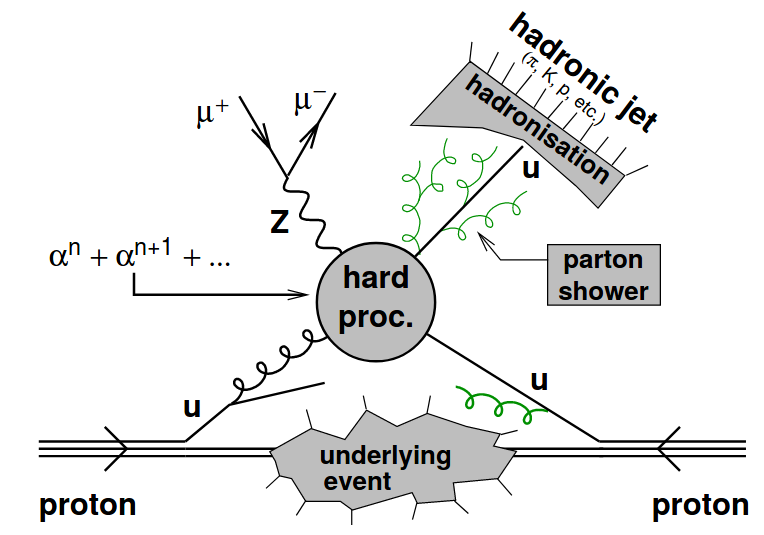
\includegraphics[width=0.5\textwidth] {Pictures/protonproton.png}\hspace{1cm}
    \caption{Example proton-proton collision with quark-gluon scattering and final state jet and Z-boson \cite{Butterworth}}.
    \label{fig:protonproton}
\end{figure}
Quarks and gluons emitted from the high energy hard scatter do not appear in the detector directly. QCD, in one of its key differences to QED, becomes stronger with larger distances. As a parton reaches high enough energy, it will begin to radiate low-energy gluons until resultant partons are able to bind into color-neutral hadrons. These hadrons are seen collimated in groups in the detector, ``jets". The energy and momentum of jets are considered reflections of the intial scattered partons. Various ``jet algorithms" can be used to determine initial parton properties as reproducibly and accurately as possible. The jet algorithm used in this analysis will be described in detail in Chapter 4. However, it is important to note that the algorithm used by all LHC experiments, anti-$k_t$, is collinear and infrared safe, unaffected by small angle and soft scatterings that occur in a parton shower. Without these qualities, perturbation theory applied to the parton shower would find infinities at high orders.

Cross-sections (denoted $\sigma$) measure the probability that a certain process will occur in the collision of two particles, in our case protons. In high energy physics, cross-sections are measured in femtobarns. A barn is the cross-sectional area of a typical nucleus, $10^{-28}$ m$^2$, and was named to describe the large target area needed in order to have direct strikes on a nucleus. The name was inspired by the expression ``could not hit the broad side of a barn''.\footnote{Inverse femtobarns ($10^{15}$ inverse barns) are used to measure the number of particle collision events per femtobarn area of a target and quantifies time-integrated luminosity.} 

Hard scattering cross-sections in hadron-hadron collisions can be calculated using the QCD factorization theorem, and to leading-order these calculations are relatively simple. In the factorization theorem, developed by Drell and Yan, deep inelastic scattering parton model processes could apply to hadron-hadron collisions. The Drell-Yan process is the production of a massive lepton pair by quark-antiquark annihilation. According to the factorization theorem, a hadronic cross-section $\sigma(ab\rightarrow \mu^+\mu^-+Y)$ could be calculated by rescaling the Drell-Yan sub-process cross-section $\hat{\sigma}$ for $\bar{q}q\rightarrow\mu^+\mu^-$ with parton distribution functions $f_{q/A}(x)$ from deep inelastic scattering \cite{Campbell}:
\begin{equation}
\sigma_{AB} = \int dx_a \, dx_b \, f_{a/A}(x_a) \, f_{b/B}(x_b) \,\hat{\sigma}{ab\rightarrow X},
\end{equation}
where $X$ represents the two resulting leptons and $ab$ the two annihilated quarks. This parton model provides good agreement with measured cross-sections and so allows understanding of particlar hard scattering processes. Predictions for some key Standard Model processes are shown in Figure \ref{fig:crosssection}. Noting the logarithmic scales, it is clear that the Higgs boson of mass 125 GeV is over an order of magnitude more numerous at the LHC than the Tevatron and that certain high mass particles like the $b$ quark and $W/Z$ bosons are abundantly produced at the LHC \cite{Campbell}. In addition, the plot shows cross-sections of particular Higgs decay modes. These will be discussed next.
 
\begin{figure}[H]
        \centering
    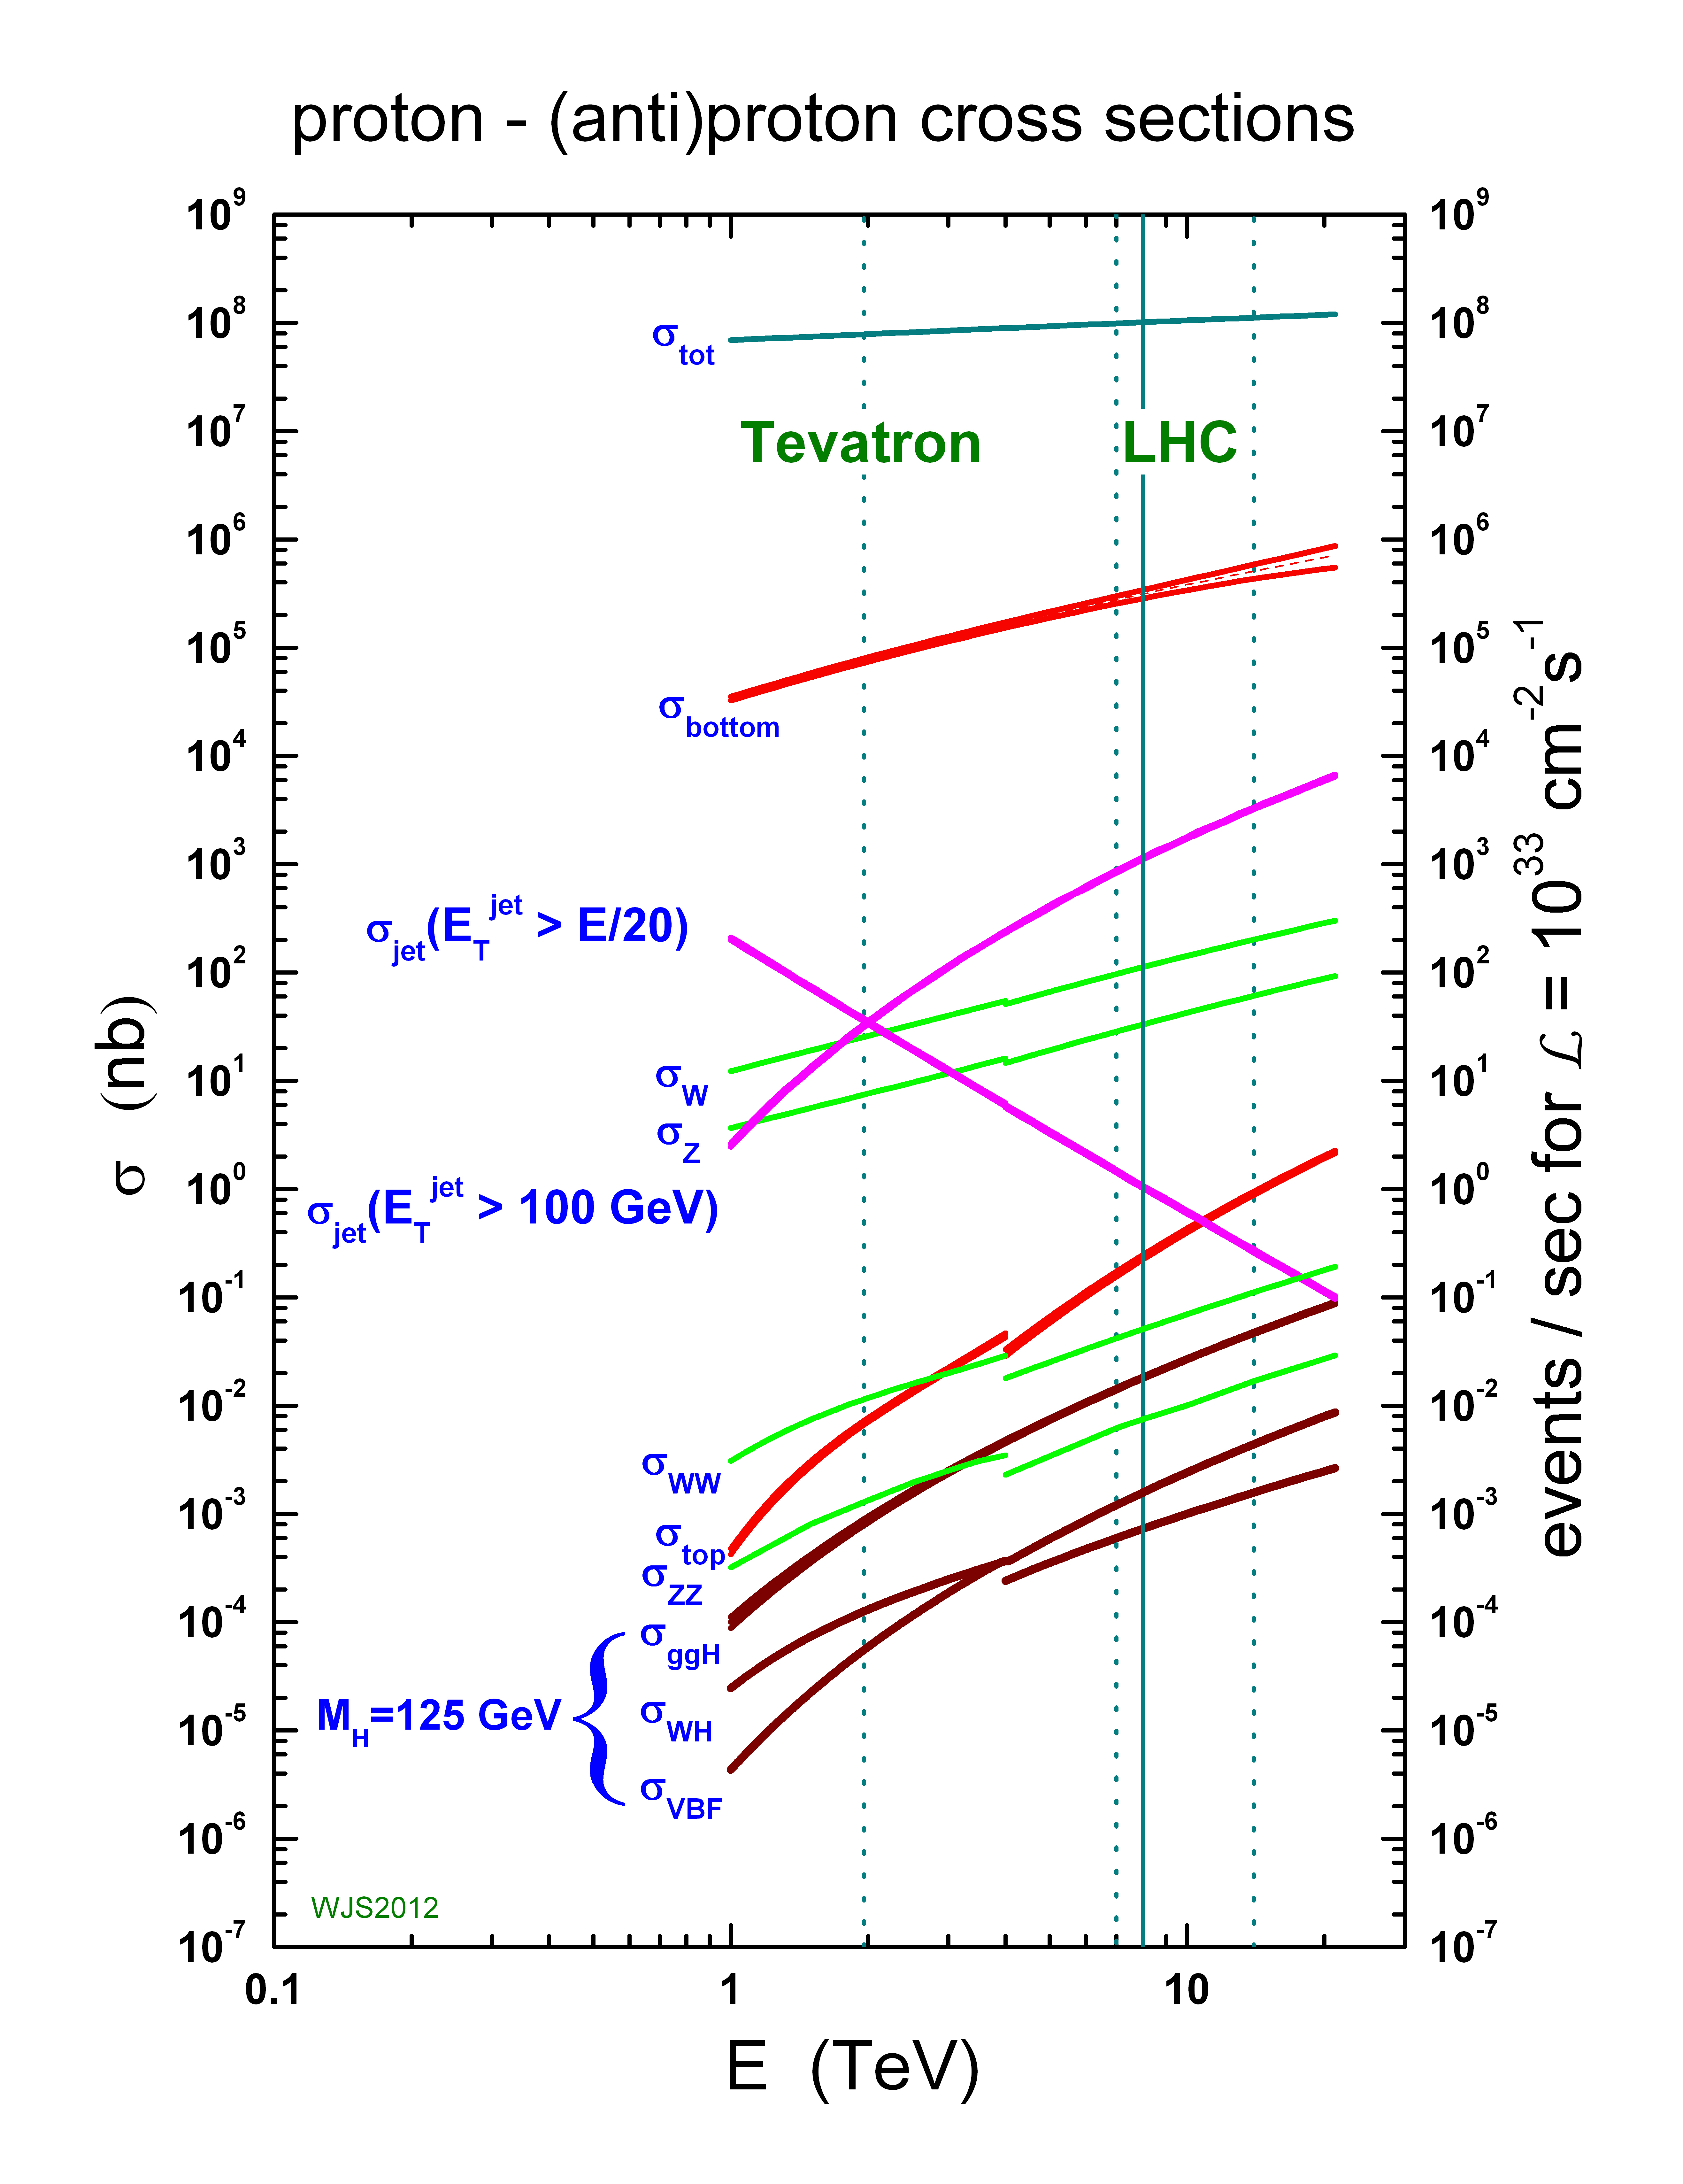
\includegraphics[width=0.5\textwidth] {Pictures/crosssections.jpg}\hspace{1cm}
    \caption{Predicted Standard Model cross-sections for the Tevatron and LHC \cite{Stirling}.}
    \label{fig:crosssection}
\end{figure}

Higgs production at the LHC occurs via four main processes: gluon-gluon fusion (ggF), vector-boson fusion, associated production with $W/Z$ bosons, and associated production with top or bottom quarks. The Feynman diagrams for these processes are shown in Figure \ref{fig:FeynmannHiggs}.  

\begin{figure}[H]
        \centering
    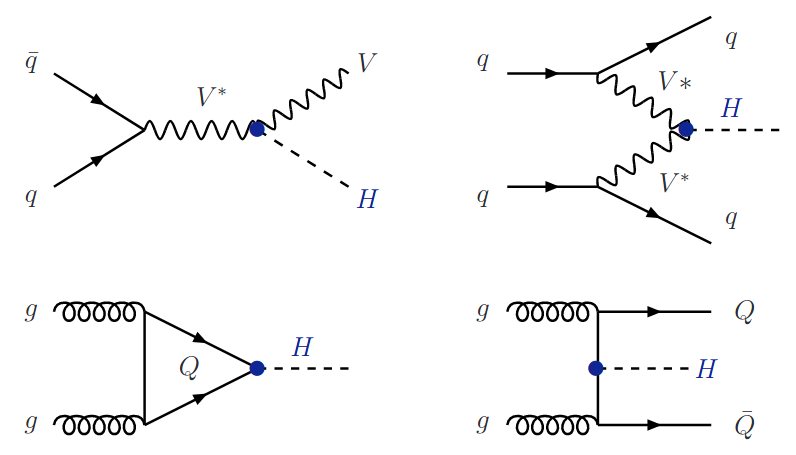
\includegraphics[width=0.5\textwidth] {Pictures/FeynmannHiggs.png}\hspace{1cm}
    \caption{Feynman diagrams for the leading Higgs boson production modes at the LHC \cite{Djouadi}.}
    \label{fig:FeynmannHiggs}
\end{figure}

The LHC Cross-section Working Group produces predictions on cross-sections, branching ratios, and pseudo-observables for the Higgs boson. Four CERN reports bring together Higgs prescriptions for current and planned LHC efforts \cite{LHCCrossSectionWG}. Figure \ref{fig:HiggsCrosssection} shows the Higgs cross-section for the main production modes as a function of the Higgs mass and the collision center-of-mass energy. The Standard Model does not predict the Higgs mass, but experimentally we know that $m_H\approx$ 125 GeV. Examining cross-section as a function of center-of-mass demonstrates the increase in statistics for events of interest that running the detector at higher energy levels can accomplish. Figure \ref{fig:HiggsCrosssection} also shows that gluon-gluon fusion Higgs production is the leading production mechanism by far. The Higgs production cross-section is currently known at next-to-next-to-leading-order (NNLO) in QCD with next-to-leading-order (NLO) EW corrections. 

The second highest production cross-section is from vector boson fusion. As seen in the Feynman diagram, two outgoing quarks are produced in the interaction. These quarks produce two hard jets in the forward region with the Higgs boson appearing between them. To leading order, VBF Higgs production is solely electroweak, and QCD corrections (calculated at NLO) have a smaller impact than in ggF. NLO EW corrections are also applied. As a result, VBF theoretical uncertainties are smaller than those on ggF. Vector boson associated Higgs production through a $W/Z$ boson are less common than VBF but also dominated by electroweak processes with a small QCD correction (NNLO). Finally, associated production with top and bottom quarks is shown, though these are quite rare and have high NLO and NNLO QCD corrections. 

\begin{figure}[H]
    \centering
    \subfloat[Higgs production cross-section by $m_H$]{{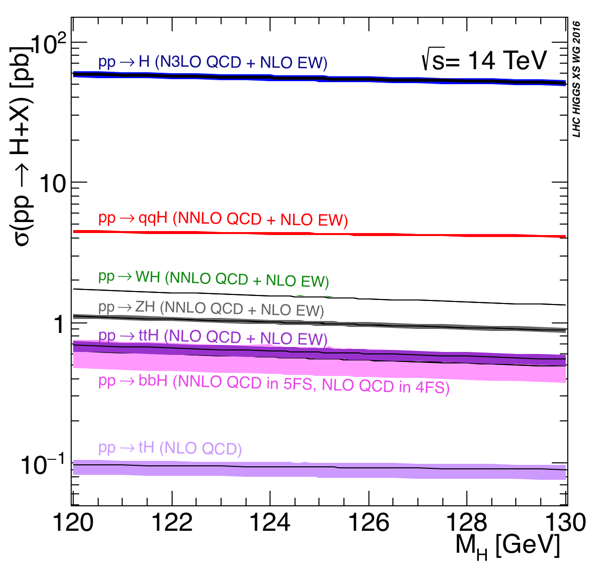
\includegraphics[width=0.4\textwidth]{Pictures/HiggsCrosssectionMH.png} }} %
    \qquad
    \subfloat[Higgs production cross-section by$\sqrt{s}$]{{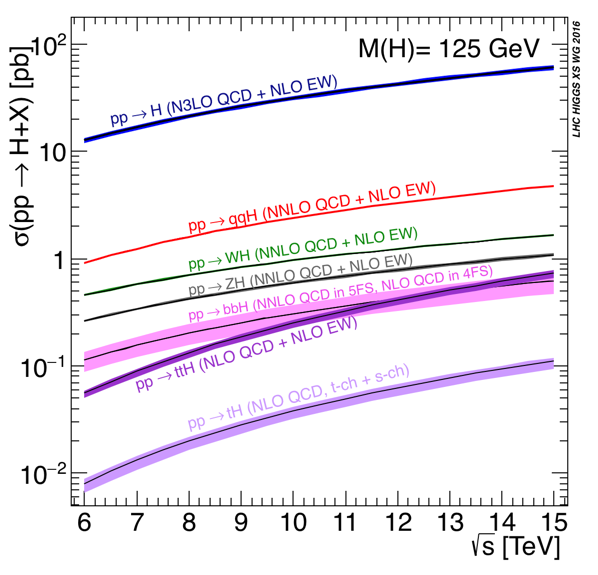
\includegraphics[width=0.4\textwidth]{Pictures/HiggsCrosssectionCOM.png} }}%
    \caption{Higgs production cross-sections over Higgs mass at center-of-mass energy 14 TeV (left) and over center-of-mass energy for a Higgs mass of 125 GeV  (right)\cite{LHCCrossSectionWG}}%
    \label{fig:HiggsCrosssection}%
\end{figure}

Theoretical uncertainties shown as colored bars in \ref{fig:HiggsCrosssection} are calculated from choice of PDFs and renormalization and factorization scales. Parton distribution functions (PDFs) are described in more detail by the PDF4LHC working group \cite{PDF4LHC15}. This group performs studies of PDFs and their predictions at the LHC and makes recommendations for methods of estimating PDF uncertainties. 

\begin{figure}[H]
        \centering
    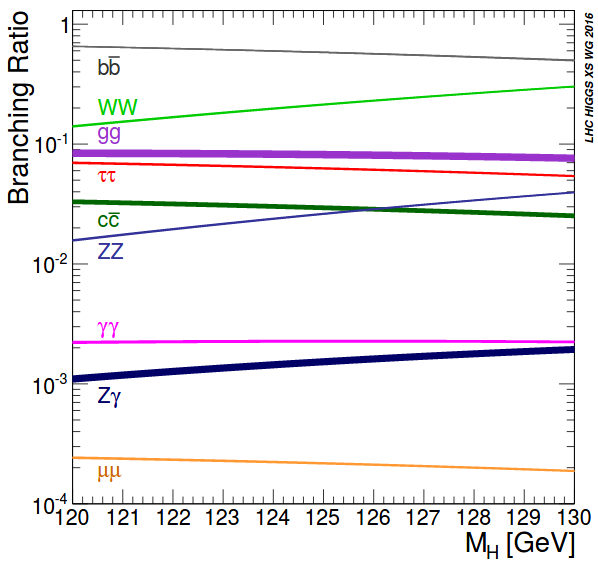
\includegraphics[width=0.45\textwidth] {Pictures/HiggsBranching.png}\hspace{1cm}
    \caption{Predicted branching ratios for the Higgs boson at the LHC as a function of Higgs mass \cite{LHCCrossSectionWG}.}
    \label{fig:HiggsBR}
\end{figure}

Since the Higgs boson couplings are directly proportional to the masses of each particle, the Higgs decays most readily into the heaviest particles possible. Figure \ref{fig:HiggsBR} shows key decay mode branching ratios near the experimentally known Higgs mass. While the branching ratios demonstrate the relative abundance of each Higgs decay, these do not translate directly into their ease of discovery or measurement. The current status of Higgs boson coupling and cross-section measurements for each decay mode will be detailed in the next section. The Higgs boson discovery was made through a combination of searches in many channels though dominated by $H\rightarrow ZZ^*$, $H\rightarrow\gamma\gamma$, and $H\rightarrow WW^*$ \cite{Higgsdiscovery}. This is because though other decay branching ratios are higher, like $H\rightarrow b\bar{b}$, the backgrounds associated with this decay are much higher. As previously mentioned, proton-proton collisions create large amounts of QCD jets that are difficult to discern from target hard QCD processes. Because of this, Higgs decays to quarks and gluons are particularly difficult and those with decays to heavy and light bosons (ZZ decays to 4 leptons, decays directly to photons, and $WW$ decays to two leptons and two neutrinos) are easier to reconstruct. As energy and integrated luminosity increased during LHC data-taking, measurements of even rare and background-heavy Higgs decay channels could be made.  This thesis focuses on the decay of $H\rightarrow W^+W^-\rightarrow \ell\nu\ell\nu$ through VBF production. In the last section of this chapter I will motivate the choice of these conditions for probing new physics beyond the SM.   

\section{Brief history of SM tests}
Here I summarize key moments in the history of the development of the Standard Model and its experimental tests. I use both Refs. \cite{Kibble} and \cite{HistoryBook} as a guide.

The history of the Standard Model could start with any number of physicists well before the formalism of the theory itself. As far back as the fifth century B.C. philosophers posited that matter is composed of discrete ``particles" in its most fundamental state. This idea was only tested beginning in the nineteenth century, when scientists were able to detect physical evidence of atoms and their structure. The first of the gauge theories, QED, was invented in the 1930s but only calculated to first order. Renormalization theory was invented simultaneously by Feynman, Schwinger, and Tomonaga in the 1940s. This made calculations of higher order QED results possible. Following this advancement, QED was verified experimentally with high precision. 

Physicists next attempted to understand and formalize the other fundamental forces, strong and weak, in the same way. Symmetries for these theories were not as easy to find as that of QED, and in 1954 the first new gauge theory for QCD was proposed by Shaw, Yang, and Mills. Though ultimately incorrect, it led to proposals for a gauge theory of weak interactions by Schwinger in 1956 (unifying weak and electromagnetic interactions with photons and massive $W^\pm$ bosons). Glashow added a fourth boson, $Z$, to the theory, but the problem of a broken symmetry necesary to give mass to the $W/Z$ bosons remained. Spontaneous symmetry breaking was a known and tested concept, but its use in the theory led to unwanted massless ``Nambu-Goldstone" bosons. Some thought this problem was inevitable in using SSB in the gauge theory. In 1964 Englert and Brout, then Higgs, and a few months later Guralnik, Hagen, and Tribble all published papers with the same conclusion---the Goldstone theorem can be applied to gauge theories and massive bosons can ``eat" the Nambu-Goldstone bosons to gain mass. This then creates a new scalar field whose particles are now termed Higgs bosons. A few years later Weinberg unified these ideas into the electroweak theory we recognize today. The theory was confirmed many times over at experiments over the next decades. 

While electroweak symmetry breaking and its implications were being understood in the 1960s, QCD was gradually being assembled. Experimental discoveries of a host of new particles led to Gell-Man and Zweig's development of a theory that these were all composed of the same three base particles, ``quarks". Han and Nambu understood that an octet of colored gauage bosons, ``gluons", mediated the strong force through color interactions. In 1973 Gross, Wilczek, and Politzer demonstrated the asymptotic freedom of QCD, its weakness at short distances which allows perturbation theory to calculate high energy interactions. The Standard Model, as it is composed of electroweak dynamics and QCD, has been remarkably predictive but there is much it does not explain, such as the existence of dark matter particles. While theoretical physicists work to expand the Standard Model (or replace it entirely), experimentalists search for deviations from Standard Model predictions, which may be the next hint of entirely new physics. 

Large amounts of experimental evidence for the predictive power of QED had amassed over time, and by the 1970s high energy accelerators at CERN, Fermilab, Brookhaven and SLAC began making first measurements of predicted electroweak and QCD observables. In 1969 physicists at SLAC collided electrons and protons and found that electron scattering behaved as though the proton was made up of point-like particles, quarks. Electroweak theory's predicted neutral weak current interaction between quarks and leptons was discovered at CERN and then Fermilab in 1973, giving evidence to electroweak unification. The $W$ and $Z$ bosons predicted by the theory with masses $\approx$ 80 GeV were discovered at the SPS at CERN. This was the first proton-antiproton collider and with a center-of-mass energy of 540 GeV, it was then the highest energy collider ever built. The collider was built for the main purpose of finding the predicted $W$ and $Z$ bosons, and it succeeded in discovering both in 1983. Electron-positron colliders like LEP at CERN and SLC at SLAC were able to produce millions of $Z$ bosons and so test electroweak predictions with high precision. The theory continued to prove extremely accurate. QCD remains more difficult to test precisely, as calculating QCD parameters theoretically is a computationally difficult task. However, evidence of QCD's accuracy has accumulated. In 1978, DESY was able to indirectly detect the first gluon. The electron-positron collider produced two quarks that formed two jets of particles with equal energy in opposite directions. QCD predicts that there would also be 3-jet events, where a gluon would be radiated from one of the scattered quarks and form a third. The strength of the strong interaction was first measured in 1978 and thereafter with more and more precision and has always followed QCD predictions. Quarks beyond the first generation (up, down) were discovered in order of increasing mass - strange first, followed by charm, then bottom, and finally in 1995 the top. Similarly, the muon was discovered well before the heavier tau-lepton which was not directly observed in the early 2000s. After these discoveries, the last Standard Model particle left undiscovered was the Higgs boson. Its mass is an input rather than a prediction to the Standard Model, but with the large amount of data taken at increasingly high energy colliders, experimentalists and theorists were confident that if it existed, its mass would be between 100 GeV and 1 TeV. In order to search for the Higgs boson, the Large Hadron Collider was planned and built at CERN. The collider and its largest all-purpose detector, ATLAS, are discussed in the next chapter. 

In 2012, the Higgs boson was discovered at the LHC in both the ATLAS and CMS detectors. After just one year of data-taking at a 7-8 TeV center-of-mass energy, combined searches in the $H\rightarrow ZZ^*\rightarrow \ell\ell\ell\ell$, $H\rightarrow \gamma\gamma$ and $H\rightarrow WW \rightarrow \ell\nu\ell\nu$ channels found a particle compatible with the Standard Model Higgs with a significance of 5.9 standard deviations at a mass close to 125 GeV. The LHC continued data-taking after the discovery with a new goal: measuring this new particle's properties with accuracy and precision. In 2015, the center-of-mass energy increased to 13 TeV and more than 20 times the data used in the first discovery has now been recorded. 

Measurements of the Higgs boson are now numerous and quite precise, but no deviations were observed from the theoretical expectation. While the Standard Model has proven a successful model of known interactions, there are many phenomena that it does not predict---from dark matter to neutrino masses. There must be physics beyond this theory. In continuing to probe new aspects of the model, the LHC may find deviations from the known forces or physics beyond the Standard Model.

The mass of the Higgs boson is measured through a combination of decay modes and in combination with CMS to be 125.10$\pm 0.14$ GeV \cite{PDG}. The latest combined Higgs cross-section measurement from ATLAS uses data from 2015-2017 and finds the production cross-sections (normalized to their Standard Model predictions) as shown in Figure \ref{fig:productioncrosssection}. Branching ratios of relevant decay modes are also measured and are shown in Figure \ref{fig:branchingratio} multiplied by their cross-sections in each relevant production mode. The differences in theoretical and systematic uncertainty for certain decays (QCD heavy VBF $H\rightarrow b\bar{b}$ in comparison to the leptonically decaying VBF $H\rightarrow WW^*$) show how discernable backgrounds play a major role in the viability of a measurement, even when the branching ratio is high \cite{HiggsCurrent}.  
\begin{figure}[H]
        \centering
    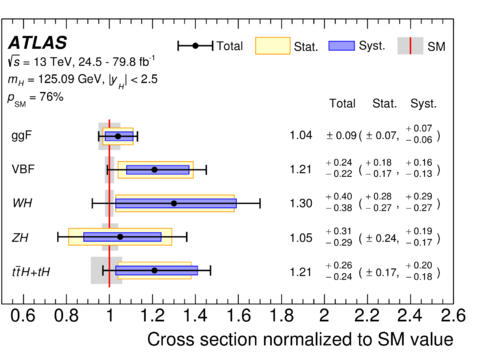
\includegraphics[width=0.5\textwidth] {Pictures/productioncrosssection.png}\hspace{1cm}
    \caption{Production cross-sections for ggF, VBF, VH, and $t\bar{t}H+tH$ normalized to their SM predictions. Total, systematic, and statistical uncertainties are shown \cite{HiggsCurrent}}
    \label{fig:productioncrosssection}
\end{figure}

\begin{figure}[H]
        \centering
    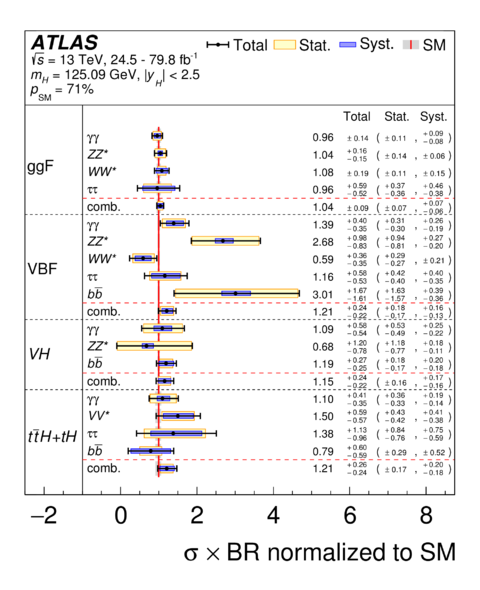
\includegraphics[width=0.5\textwidth] {Pictures/branchingratio.png}\hspace{1cm}
    \caption{Branching ratios for measured Higgs decays normalized to their SM predictions. Total, systematic, and statistical uncertainties are shown \cite{HiggsCurrent}}
    \label{fig:branchingratio}
\end{figure}
This thesis details my work on the fiducial cross-section measurement of VBF $H\rightarrow WW^*\rightarrow\ell\nu\ell\nu$ decays. The clear sign of VBF Higgs production (2 jets recoiling in opposite high $\eta$ directions, combined with the leptonically decaying $W$ bosons) gives the decay a distinctive signature. This channel can be measured with high accuracy which may allow small deviations from theory to be visible. In addition, the measurement is made with the goal of eventual differential cross-section measurements, which can probe higher order perturbative contributions to QCD or EW. Details on the particular motivations for this thesis' analysis will be outlined in the next section. The last ATLAS $H\rightarrow WW^*$ differential measurement was published in 2016 with 20.3 fb$^{-1}$ at center-of-mass energy 8 TeV and measured only ggF Higgs boson production differential cross-sections \cite{HiggsDifferential}. 

%This will also to be the first ATLAS measurement focussing on VBF Higgs differential cross-sections. 

\section{Measurement motivation}
There are many reasons why the VBF $H\rightarrow\ell\nu\ell\nu$ channel is particularly interesting to investigate. Since the $W$ bosons decay leptonically, they create a clear signal in the detector which allows for a precise reconstruction of the hard processes. Further, the VBF production mode has a similarly clear signal with the two jets accompanying the decaying $W$ bosons with a high $\eta$ separation. The pseudorapidity of these jets and the rapidity between them are particularly sensitive to the electroweak symmetry breaking mechanism, so a differential cross-section measurement over these variables (along with other detailed and motivated in further sections) tests the Higgs mechanism. In 2019, VBF $H\rightarrow WW^* \rightarrow \ell\nu\ell\nu$ cross-sections were measured in 2015-2016 data with an experimental uncertainty of $\approx50\%$ \cite{Aaboud_2019}. This new measurement uses all data recorded from 2015-2018, with a factor of 3.9 times higher statistics. This VBF $H\rightarrow WW$ fiducial cross-section measurement uses new analysis techniques and improvements in theoretical calculations as well as higher statistics to make an accurate probe of new physics within the electroweak symmetry breaking mechanism.

This thesis focuses on the VBF $H\rightarrow WW$ fiducial cross-section measurement, but this measurement is the first piece to a larger goal beyond the scope of my Ph.D. Our group plans to make a simultaneous measurement of VBF $H\rightarrow WW$ and VBF $W+$jets fiducial and differential cross-sections. The VBF $W+jj$ production cross-section is sensitive to the $WWV$ vertex. In vector boson scattering, we expect (with minimal assumptions) that new physics ought to be at a scale above the current experiment. Effects from this type of new physics would simultaneously affect $HWW$ and $WWV$ vertices. In particular, dimension-6 operators affect VBF Higgs mechanisms and VBF $W$ production, while the interplay of VBF and VBS mechanisms allows for the probe of dimension-6 and dimension-8 operators. Measuring fiducial and differential cross-section ratios (of VBF Higgs and $Wjj$) enhances sensitivity to new physics because any new phenomena that simultaneously affect both vertices are suppressed and so sensitivity to the phenomena affecting just the $WWV$ vertex (for example, anamolous quadruple-gauge couplings) is enhanced.  VBF Higgs and $Wjj$ productions are also characterized by final-states with two jets with similar kinematics. Because of this, the ratio of cross-sections measurement allows for the cancellations of correlated systematic uncertainties. As both process are characterized by large ($10\%-20\%$) jet-related uncertainties, a reduction via the ratio cancellation would greatly improve the sensitivity to the VBF Higgs process and to the search for new phenomena. This VBF $HWW$ measurement is the first part of the ratio of fiducial differential cross-sections for VBF $HWW$ and $Wjj$, which will set limits on parameters, benefiting from enhanced sensitivity through the cancellation of correlated uncertainties. 
